\documentclass[useAMS,usenatbib,referee]{biom}
%\documentclass[useAMS,usenatbib,referee]{biom}
%
%
%  Papers submitted to Biometrics should ALWAYS be prepared
%  using the referee option!!!!
%
%
% If your system does not have the AMS fonts version 2.0 installed, then
% remove the useAMS option.
%
% useAMS allows you to obtain upright Greek characters.
% e.g. \umu, \upi etc.  See the section on "Upright Greek characters" in
% this guide for further information.
%
% If you are using AMS 2.0 fonts, bold math letters/symbols are available
% at a larger range of sizes for NFSS release 1 and 2 (using \boldmath or
% preferably \bmath).
%
% The usenatbib command allows the use of Patrick Daly's natbib package for
% cross-referencing.
%
% If you wish to typeset the paper in Times font (if you do not have the
% PostScript Type 1 Computer Modern fonts you will need to do this to get
% smoother fonts in a PDF file) then uncomment the next line
% \usepackage{Times}
%%%%% AUTHORS - PLACE YOUR OWN MACROS HERE %%%%%

\usepackage[figuresright]{rotating}
\usepackage{tikz}
\usepackage{amsmath}
\usepackage[hyphens]{url} % not crucial - just used below for the URL
\usepackage{hyperref}
\usepackage[utf8]{inputenc}
\usepackage{graphicx}
\usepackage{longtable}
\usepackage{booktabs}
%% \raggedbottom % To avoid glue in typesetteing, sbs>>

% Pandoc syntax highlighting
\usepackage{color}
\usepackage{fancyvrb}
\newcommand{\VerbBar}{|}
\newcommand{\VERB}{\Verb[commandchars=\\\{\}]}
\DefineVerbatimEnvironment{Highlighting}{Verbatim}{commandchars=\\\{\}}
% Add ',fontsize=\small' for more characters per line
\usepackage{framed}
\definecolor{shadecolor}{RGB}{248,248,248}
\newenvironment{Shaded}{\begin{snugshade}}{\end{snugshade}}
\newcommand{\AlertTok}[1]{\textcolor[rgb]{0.94,0.16,0.16}{#1}}
\newcommand{\AnnotationTok}[1]{\textcolor[rgb]{0.56,0.35,0.01}{\textbf{\textit{#1}}}}
\newcommand{\AttributeTok}[1]{\textcolor[rgb]{0.77,0.63,0.00}{#1}}
\newcommand{\BaseNTok}[1]{\textcolor[rgb]{0.00,0.00,0.81}{#1}}
\newcommand{\BuiltInTok}[1]{#1}
\newcommand{\CharTok}[1]{\textcolor[rgb]{0.31,0.60,0.02}{#1}}
\newcommand{\CommentTok}[1]{\textcolor[rgb]{0.56,0.35,0.01}{\textit{#1}}}
\newcommand{\CommentVarTok}[1]{\textcolor[rgb]{0.56,0.35,0.01}{\textbf{\textit{#1}}}}
\newcommand{\ConstantTok}[1]{\textcolor[rgb]{0.00,0.00,0.00}{#1}}
\newcommand{\ControlFlowTok}[1]{\textcolor[rgb]{0.13,0.29,0.53}{\textbf{#1}}}
\newcommand{\DataTypeTok}[1]{\textcolor[rgb]{0.13,0.29,0.53}{#1}}
\newcommand{\DecValTok}[1]{\textcolor[rgb]{0.00,0.00,0.81}{#1}}
\newcommand{\DocumentationTok}[1]{\textcolor[rgb]{0.56,0.35,0.01}{\textbf{\textit{#1}}}}
\newcommand{\ErrorTok}[1]{\textcolor[rgb]{0.64,0.00,0.00}{\textbf{#1}}}
\newcommand{\ExtensionTok}[1]{#1}
\newcommand{\FloatTok}[1]{\textcolor[rgb]{0.00,0.00,0.81}{#1}}
\newcommand{\FunctionTok}[1]{\textcolor[rgb]{0.00,0.00,0.00}{#1}}
\newcommand{\ImportTok}[1]{#1}
\newcommand{\InformationTok}[1]{\textcolor[rgb]{0.56,0.35,0.01}{\textbf{\textit{#1}}}}
\newcommand{\KeywordTok}[1]{\textcolor[rgb]{0.13,0.29,0.53}{\textbf{#1}}}
\newcommand{\NormalTok}[1]{#1}
\newcommand{\OperatorTok}[1]{\textcolor[rgb]{0.81,0.36,0.00}{\textbf{#1}}}
\newcommand{\OtherTok}[1]{\textcolor[rgb]{0.56,0.35,0.01}{#1}}
\newcommand{\PreprocessorTok}[1]{\textcolor[rgb]{0.56,0.35,0.01}{\textit{#1}}}
\newcommand{\RegionMarkerTok}[1]{#1}
\newcommand{\SpecialCharTok}[1]{\textcolor[rgb]{0.00,0.00,0.00}{#1}}
\newcommand{\SpecialStringTok}[1]{\textcolor[rgb]{0.31,0.60,0.02}{#1}}
\newcommand{\StringTok}[1]{\textcolor[rgb]{0.31,0.60,0.02}{#1}}
\newcommand{\VariableTok}[1]{\textcolor[rgb]{0.00,0.00,0.00}{#1}}
\newcommand{\VerbatimStringTok}[1]{\textcolor[rgb]{0.31,0.60,0.02}{#1}}
\newcommand{\WarningTok}[1]{\textcolor[rgb]{0.56,0.35,0.01}{\textbf{\textit{#1}}}}

% tightlist command for lists without linebreak
\providecommand{\tightlist}{%
  \setlength{\itemsep}{0pt}\setlength{\parskip}{0pt}}



%%%%%%%%%%%%%%%%%%%%%%%%%%%%%%%%%%%%%%%%%%%%%%%%

\setcounter{footnote}{2}

\title[]{Average treatment effect of cholesterol-lowering medication and
average systolic blood pressure (SBP), mm Hg.}

\author{ Jackson
Gazin \email{\href{mailto:gazij22@wfu.edu}{\nolinkurl{gazij22@wfu.edu}}} \\ Department
of Statistics, Wake Forest University  \and
		 Ashley
Mullan \email{\href{mailto:mullae22@wfu.edu}{\nolinkurl{mullae22@wfu.edu}}} \\ Department
of Statistics, Wake Forest University  \and
		 Anh
Nguyen \email{\href{mailto:nguyp22@wfu.edu}{\nolinkurl{nguyp22@wfu.edu}}} \\ Department
of Statistics, Wake Forest University 
	   }


\begin{document}


\date{{\it Received Dec} 2023}

\pagerange{\pageref{firstpage}--\pageref{lastpage}} \pubyear{2023}

\volume{0}
\artmonth{January}
\doi{0000-0000-0000}

%  This label and the label ``lastpage'' are used by the \pagerange
%  command above to give the page range for the article

\label{firstpage}

%  pub the summary here

\begin{abstract}
We investigate the average treatment effect among the treated (ATT) of
cholesterol-lowering medication on the mean systolic blood pressure (mm
Hg). Using data from the National Health and Nutrition Examination
Survey (NHANES), we fit a propensity score model to estimate the ATT
among adults living in the United States of America.
\end{abstract}

%
%  Please place your key words in alphabetical order, separated
%  by semicolons, with the first letter of the first word capitalized,
%  and a period at the end of the list.
%

\begin{keywords}
cholesterol-lowering medicationsystolic blood pressureblood pressure
control.
\end{keywords}

\maketitle

\hypertarget{intro}{%
\section{Introduction}\label{intro}}

Controlling blood pressure (BP) reduces the risk for cardiovascular
disease. However, the prevalence of BP control (i.e., systolic BP
\textless{} 140 and diastolic BP \textless{} 90) among US adults with
hypertension has decreased since 2013. We invite teams to analyze
publicly available data from US adults to help identify potential causes
or correlates of worsening BP control among US adults with hypertension
over the past decade, as this may allow for development of effective
interventions to help control BP and prevent cardiovascular disease.

\hypertarget{methods}{%
\section{Materials and methods}\label{methods}}

\hypertarget{data}{%
\subsection{Data}\label{data}}

The National Health and Nutrition Examination Survey (NHANES) combines
interviews and physical examinations to assess the health and
nutritional status of adults and children in the United States of
America. The program started in the early 1960s and has been conducted
every two years since 1999. The survey samples from a nationally
representative 5,000 persons each year. The participants are located in
counties across the country, 15 of which are visited each year. The
interview asks questions about demographic, socioeconomic, dietary, and
health-related questions. The examination consists of medical, dental,
physiological measurements, and laboratory tests.

The NHANES dataset we are using can be downloaded from \textbf{cite} .
The dataset contains information from the survey from 1999 to 2020 with
a sample of 59,799 rows and 111 chosen columns. Each row is a
noninstitutionalized US adults participated in the survey between 1999
and 2020. The columns contain information about demographics, blood
pressure levels, hypertension status, antihypertensive medication usage,
and co-morbidities.

For this analysis, we had 38977 rows with NA values. We decided to deal
with this by removing all the na values. We decided this was preferable
to removing certain columns since we were still left with 20,822 data
points which is still an extremely large data set.

\hypertarget{statistical-methods}{%
\subsection{Statistical methods}\label{statistical-methods}}

We fitted a propensity score model with ``Total cholesterol'' in mg/dL
as our explanatory variable since this was the only variable, and
``taking cholesterol medication'' as our response variable, as it
represents our exposure variable. We employed a Logistic Regression
model for the propensity score model.

Subsequently, we used the propensity score model to fit our outcome
model, estimating the average treatment effect among the treated. We
utilized a linear regression model with ``cholesterol medication'' as
our explanatory variable and ``Systolic blood pressure (SBP)'' in mm Hg
as our response variable.

To assess the appropriateness of our propensity score model and proceed
with our final model, we employed weighted mirrored histograms, ECDF
plots, and Love Plots.

\hypertarget{exploratory-data-analysis}{%
\subsubsection{Exploratory data
analysis}\label{exploratory-data-analysis}}

\hypertarget{modeling}{%
\subsubsection{Modeling}\label{modeling}}

\hypertarget{results-results}{%
\section{Results \{\$results\}}\label{results-results}}

\hypertarget{study-population}{%
\subsection{Study population}\label{study-population}}

We aim answer our causal question by fitting an average treatment effect
among the treated. Our causal question is as follows: Among those who
take cholesterol lowering medication, does taking this cholesterol
lowering medication change their systolic blood pressure?

\hypertarget{propensity-score-model-and-diagnostics}{%
\subsection{Propensity score model and
Diagnostics}\label{propensity-score-model-and-diagnostics}}

We fitted a propensity score model with ``total cholesterol'' in mg/dL
as our explanatory variable and ``taking cholesterol medication'' as our
response variable. We employed a Logistic Regression model for this
purpose. Subsequently, we examined a Mirrored Histogram of our
propensity scores for both exposure groups. The table below demonstrates
significant overlap in propensity scores across both groups, indicating
very little evidence of a positivity violation in our model, which is
promising.

Next, we used our propensity score model to generate weights for the
average treatment effect among the treated (ATT), aligning with our
causal question. To assess the appropriateness of our propensity score
model and the resulting weights, we created a Weighted Mirror Histogram
of our propensity scores. As shown below, we achieved sufficient balance
between the exposed and unexposed groups. Furthermore, the distribution
of the unexposed group now resembles that of the exposed group, which is
the desired outcome when using ATT weights.

We also generated a love plot, displaying the standardized mean
difference changes for the exposed and unexposed groups regarding our
``total cholesterol'' variable in both unweighted and weighted data. As
expected, our weighted data exhibit a standardized mean difference of 0
for the ``total cholesterol'' variable, which is ideal and allows us to
proceed.

Finally, we created a weighted empirical cumulative distribution
function (eCDF) plot for our continuous variable, ``total cholesterol.''
As shown below, the Weighted ECDF plot indicates balance not only in the
mean across exposure groups but also across their respective
distributions. No changes are required for our model, and we can now
proceed to estimate our average treatment effect among the treated.

\hypertarget{average-treatment-effect-among-the-treated}{%
\subsection{Average treatment effect among the
treated}\label{average-treatment-effect-among-the-treated}}

We estimated the average treatment effect of taking cholesterol-lowering
medication. Our findings indicate that, on average, individuals who take
cholesterol-lowering medication experience an increase of 9.26 mm Hg in
their Systolic Blood Pressure (SBP). We are 95 percent confident that
the average effect of taking this medication on SBP falls within the
range of at least 8.578 mm Hg to at most 9.941 mm Hg. Additionally, we
conducted a sensitivity analysis to account for the possibility that our
Directed Acyclic Graph (DAG) might not include all potential confounding
variables. In this analysis, we calculated the necessary relationship
between an unmeasured confounder and the change in weight required to
shift the lower bound of the confidence interval to the null hypothesis
level (5\%). We considered exposure confounder effects of sizes 0.05,
0.10, and 0.15, which would necessitate confounder-outcome effects of
172, 85, and 57, respectively, to influence the interval. The smallest
of these values, 57, is over 6 times greater than the estimated
treatment effect. Therefore, it is reasonable to conclude that the
Average Treatment Effect (ATT) we computed is robust against potential
confounding factors.

\hypertarget{discussion}{%
\section{Discussion}\label{discussion}}

\hypertarget{supplement}{%
\section{Supplementary information}\label{supplement}}

The data can be downloaded from GitHub or accessed via the
cardioStatsUSA R package. For both the file and information about the R
package, see \url{https://github.com/jhs-hwg/cardioStatsUSA}.

All code for the analysis can be accessed at \textbf{link github}

\hypertarget{acknowledge}{%
\section{Acknowledgement}\label{acknowledge}}

\hypertarget{sec:1}{%
\section{Section title}\label{sec:1}}

Text with citations by \citet{heagerty2000time},
\citep{pepe2003statistical}.

\hypertarget{sec:2}{%
\subsection{Subsection title}\label{sec:2}}

as required \citep{hoerl1970ridge, zou2005regularization}. Don't forget
to give each section and subsection a unique label (see Sect.
\ref{sec:1}).

\hypertarget{paragraph-headings}{%
\paragraph{Paragraph headings}\label{paragraph-headings}}

Use paragraph headings as needed.

\hypertarget{equations}{%
\subsection{Equations}\label{equations}}

Here is an equation:

\[ f_{X}(x) = \left(\frac{\alpha}{\beta}\right)\left(\frac{x}{\beta}\right)^{\alpha-1}e^{-\left(\frac{x}{\beta}\right)^{\alpha}}; \alpha,\beta,x > 0 \]

Here is another: \begin{align}
a^2+b^2=c^2
\end{align}

Inline equations: \(\sum_{i = 2}^\infty\{\alpha_i^\beta\}\)

\hypertarget{figures-and-tables}{%
\section{Figures and tables}\label{figures-and-tables}}

\hypertarget{figures-coming-from-r}{%
\subsection{Figures coming from R}\label{figures-coming-from-r}}

\hypertarget{normal-figure-embedded-in-text}{%
\paragraph{Normal figure embedded in
text}\label{normal-figure-embedded-in-text}}

\begin{verbatim}
## Warning in plot.formula(runif(25) ~ runif(25)): the formula 'runif(25) ~
## runif(25)' is treated as 'runif(25) ~ 1'
\end{verbatim}

\begin{figure}
\centering
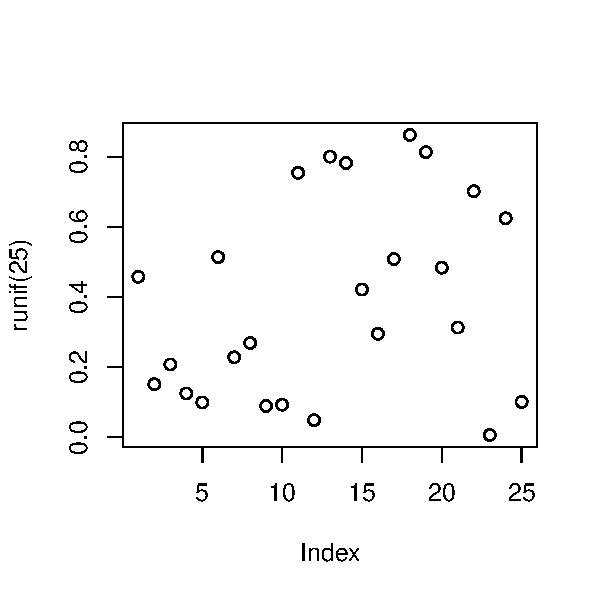
\includegraphics{final-project_files/figure-latex/fig2-1.pdf}
\caption{Output from \texttt{pdf()}}
\end{figure}

\clearpage

\hypertarget{tables-coming-from-r}{%
\subsection{Tables coming from R}\label{tables-coming-from-r}}

\begin{Shaded}
\begin{Highlighting}[]
\FunctionTok{print}\NormalTok{(xtable}\SpecialCharTok{::}\FunctionTok{xtable}\NormalTok{(}\FunctionTok{head}\NormalTok{(mtcars)[,}\DecValTok{1}\SpecialCharTok{:}\DecValTok{4}\NormalTok{], }
\AttributeTok{caption =} \StringTok{"Caption centered under table"}\NormalTok{, }\AttributeTok{label =} \StringTok{"tab1"}\NormalTok{), }
\AttributeTok{comment =} \ConstantTok{FALSE}\NormalTok{, }\AttributeTok{timestamp =} \ConstantTok{FALSE}\NormalTok{, }\AttributeTok{caption.placement =} \StringTok{"top"}\NormalTok{)}
\end{Highlighting}
\end{Shaded}

\begin{table}[ht]
\centering
\caption{Caption centered under table} 
\label{tab1}
\begin{tabular}{rrrrr}
  \hline
 & mpg & cyl & disp & hp \\ 
  \hline
Mazda RX4 & 21.00 & 6.00 & 160.00 & 110.00 \\ 
  Mazda RX4 Wag & 21.00 & 6.00 & 160.00 & 110.00 \\ 
  Datsun 710 & 22.80 & 4.00 & 108.00 & 93.00 \\ 
  Hornet 4 Drive & 21.40 & 6.00 & 258.00 & 110.00 \\ 
  Hornet Sportabout & 18.70 & 8.00 & 360.00 & 175.00 \\ 
  Valiant & 18.10 & 6.00 & 225.00 & 105.00 \\ 
   \hline
\end{tabular}
\end{table}

Table \ref{tab1} shows these numbers. Some of those numbers are plotted
in Figure \ref{fig:fig1}.

\begin{Shaded}
\begin{Highlighting}[]
\FunctionTok{head}\NormalTok{(mtcars[,}\DecValTok{1}\SpecialCharTok{:}\DecValTok{4}\NormalTok{])}
\end{Highlighting}
\end{Shaded}

\begin{verbatim}
##                    mpg cyl disp  hp
## Mazda RX4         21.0   6  160 110
## Mazda RX4 Wag     21.0   6  160 110
## Datsun 710        22.8   4  108  93
## Hornet 4 Drive    21.4   6  258 110
## Hornet Sportabout 18.7   8  360 175
## Valiant           18.1   6  225 105
\end{verbatim}


\bibliographystyle{biom}
\bibliography{bibliography.bib}


\label{lastpage}


\end{document}
